
%%%%%%%%%%%%%%%%%%%% author.tex %%%%%%%%%%%%%%%%%%%%%%%%%%%%%%%%%%%
%
% sample root file for your "contribution" to a proceedings volume
%
% Use this file as a template for your own input.
%
%%%%%%%%%%%%%%%% Springer %%%%%%%%%%%%%%%%%%%%%%%%%%%%%%%%%%


\documentclass{svproc}
%
% RECOMMENDED %%%%%%%%%%%%%%%%%%%%%%%%%%%%%%%%%%%%%%%%%%%%%%%%%%%
%
\usepackage{graphicx}
\usepackage{hyperref}
\usepackage{amsmath}% http://ctan.org/pkg/amsmath
\newcommand{\thickhat}[1]{\mathbf{\hat{\text{$#1$}}}}
\newcommand{\thickbar}[1]{\mathbf{\bar{\text{$#1$}}}}
\newcommand{\thicktilde}[1]{\mathbf{\tilde{\text{$#1$}}}}
\usepackage{subfig}
\usepackage{cite}
\usepackage{amsmath}
\usepackage{multicol}
\usepackage{array}
\usepackage{float}
\newcolumntype{x}[1]{>{\centering\arraybackslash\hspace{0pt}}p{#1}}

% to typeset URLs, URIs, and DOIs
\usepackage{url}
\def\UrlFont{\rmfamily}


%\usepackage[english,spanish]{babel}
%\AtBeginDocument{\selectlanguage{spanish}}
%\renewcommand{\figurename}{Figura}
%\renewcommand{\refname}{Referencias}
%\renewcommand{\tablename}{Tabla}

\begin{document}
\mainmatter              % start of a contribution
%
\title{SplitThreader: Exploration and analysis of rearrangements in cancer genomes}
%
\titlerunning{SplitThreader}  

\author{Vicente Machaca Arceda }
\authorrunning{M.A Machaca et al.} 
\tocauthor{M.A. Machaca Arceda}
\institute{Universidad Nacional de San Agustín, Arequipa-Perú,\\
\email{vmachacaa@unsa.edu.pe}} 


\maketitle             

\begin{abstract}

Phylogenetics analysis is a very important task in Bioinformatics, we could learn about evolution, the relation between specimens. Nevertheless, a phylogenetics tree depends on the similarity analysis performed before. This similarity analysis is based on sequence alignment methods like  BLAST and CLUSTALW, but they are too slow and we need other algorithms to process similarity between sequences. In this work, we present an analysis of four alignment-free algorithms based on the image texture computed from a sequence. We compared first-order statistics, gray level co-occurrence matrix, local binary patterns, and multi-resolution local binary patterns. Moreover, we used several mapping functions for each base. Then, we compared which of these algorithms were more similar to CLUSTALW. Finally, we got that first-order statistics is the method that is more likely to CLUSTALW with the advantage of having a low computational cost.

\keywords{Similarity analysis, Phylogentics trees, alignment-free methods, image textures.}
\end{abstract}


%- Introducción: Contexto, Problema, Objetivo o Pregunta de Principal que el
%proyecto pretende dar respuesta.
%- Data Set: Presentación del conjunto de datos con alguna visualización de los
%mismos. Informar cualquier dificultad o problema asociado con el conjunto de
%datos, incluidos los análisis fallidos.
%- Marco Teórico: Breve descripción de los métodos utilizados para el proyecto y
%sus fundamentos.
%- Trabajos Relacionados: Principales trabajos relevantes que intentan resolver
%el problema planteado

%- Propuesta: Presentación de cómo se ha realizado el análisis real. Descripción
%de la arquitectura o flujo de información (pipeline) de la propuesta de solución al
%problema planteado. Incluir los algoritmos, programas o paquetes y su
%utilización.
%- Evaluación: Presentación de los resultados y su interpretación - gráficos muy
%recomendable.
%- Conclusiones: Conclusiones finales del estudio, tanto de fracasos como
%aciertos. En caso de falla, debería ser discutido los motivos y recomendaciones
%para el futuro que ayudarían a evitar los problemas encontrados.

%%%%%%%%%%%%%%%%%%%%%%%%%%%%%%%%%%%%%%%%%%%%%%%%%%%%%%%%%%%%%%%%%%%%%%%%%%%%%%%%%%%%%
%%%%%%%%%%%%%%%%%%%%%%%%%%%%%%%%%%%%%%%%%%%%%%%%%%%%%%%%%%%%%%%%%%%%%%%%%%%%%%%%%%%%%
\section{Introduction} 
%%%%%%%%%%%%%%%%%%%%%%%%%%%%%%%%%%%%%%%%%%%%%%%%%%%%%%%%%%%%%%%%%%%%%%%%%%%%%%%%%%%%%
%%%%%%%%%%%%%%%%%%%%%%%%%%%%%%%%%%%%%%%%%%%%%%%%%%%%%%%%%%%%%%%%%%%%%%%%%%%%%%%%%%%%%

Genomics data has growth up exponentially, for example in 2009, they reached about 0.8 ZB, moreover in 2020 they reached about 40 ZB \cite{prabahar2016perspectives}. Furthermore, cancer related data are generated from: gene expression data (Microarray), NGS data, protein–protein interaction (PPI), pathway annotation data y gene ontology (GO). These data are important for research in cancer diagnosis and treatment. Big data resources allow researchers to observe large retrospective, and heterogeneous data of cancer patients \cite{berman2013principles}.\\

For instance, the human genome is made of approximately 3.2 billions bp of DNA \cite{archibald2018genomics}. The HIV-1 genome is made of 20k bp of DNA, meanwhile the COVID-19 is made of 32k bp \cite{randhawa2020machine}. Additionally, there are approximately 19000 to 25000 genes (no one knows for sure) \cite{archibald2018genomics}. Finally, human genes have dozens of introns, each of which can be tens of thousands of nucleotides. Distinguishing exons from introns and other forms of non-coding DNA is challenging \cite{archibald2018genomics}. This lack of information, makes difficult the research in cancer genomics.\\

Moreover, genomic instability is one of the hallmarks of cancer \cite{hanahan2011hallmarks,hastings2009mechanisms},	resulting in a widespread copy number changes, structural variants and chromosome-scale rearrangements \cite{nattestad2016splitthreader}. Furthermore, copy number variants and gene fusions are common drivers in cancer \cite{shlien2009copy, mitelman2007impact}. In this context, it is very important to detect these structural variants, but the available algorithms for identifying gene fusions do not have perfect specificity (false positive rate)  and they require a joint analysis of genomic and transcriptomic data. Moreover, rearrangements variants are difficult to study because of the sheer complexity of rearrangements, which often include adjacencies between distant regions of a chromosome or even between unrelated chromosomes \cite{nattestad2016splitthreader}.  \\

In this work, we reviewed and replicated the tool SplitThreader \cite{nattestad2016splitthreader}. It is an open source interactive web application for analysis and visualization of genomics rearrangements and copy number variation in cancer genomes. \\


%%%%%%%%%%%%%%%%%%%%%%%%%%%%%%%%%%%%%%%%%%%%%%%%%%%%%%%%%%%%%%%%%%%%%%%%%%%%%%%%%%%%%
%%%%%%%%%%%%%%%%%%%%%%%%%%%%%%%%%%%%%%%%%%%%%%%%%%%%%%%%%%%%%%%%%%%%%%%%%%%%%%%%%%%%%
%\section{Data} 
%%%%%%%%%%%%%%%%%%%%%%%%%%%%%%%%%%%%%%%%%%%%%%%%%%%%%%%%%%%%%%%%%%%%%%%%%%%%%%%%%%%%%
%%%%%%%%%%%%%%%%%%%%%%%%%%%%%%%%%%%%%%%%%%%%%%%%%%%%%%%%%%%%%%%%%%%%%%%%%%%%%%%%%%%%%


%%%%%%%%%%%%%%%%%%%%%%%%%%%%%%%%%%%%%%%%%%%%%%%%%%%%%%%%%%%%%%%%%%%%%%%%%%%%%%%%%%%%%
%%%%%%%%%%%%%%%%%%%%%%%%%%%%%%%%%%%%%%%%%%%%%%%%%%%%%%%%%%%%%%%%%%%%%%%%%%%%%%%%%%%%%
\section{Concepts} 
%%%%%%%%%%%%%%%%%%%%%%%%%%%%%%%%%%%%%%%%%%%%%%%%%%%%%%%%%%%%%%%%%%%%%%%%%%%%%%%%%%%%%
%%%%%%%%%%%%%%%%%%%%%%%%%%%%%%%%%%%%%%%%%%%%%%%%%%%%%%%%%%%%%%%%%%%%%%%%%%%%%%%%%%%%%

In this section, we present the most relevant concepts related to bioinformatics and cancer genomics.

\subsection{Genomics data}

``DNA is abbreviation of deoxyribonucleic acid, organic chemical of complex molecular structure that is found in all prokaryotic and eukaryotic cells and in many viruses. DNA codes genetic information for the transmission of inherited traits'' \cite{dna_definition}. Moreover, the term genomics is used to refer the sum total of DNA in cells \cite{archibald2018genomics}. For instance, in Figure \ref{fig:dna}, we present a piece of COVID-19 DNA (genome) in FASTA format. DNA data is just a string of four characters: A, C, G, T that represent the nitrogen bases Adenine, Cytosine, Guanine and Thymine respectively. Unfortunately, this data is not 100\% accurate and for a single human genome, it could reaches about 4 GB (3.2 billion bases).    


\begin{figure}[H]
	\centering
	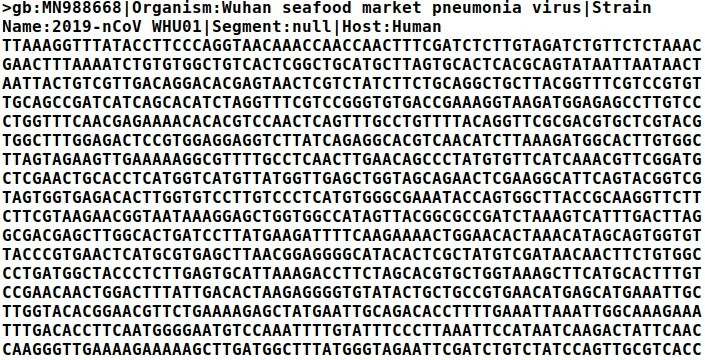
\includegraphics[width=0.6\textwidth]{img/splitthreader/dna}
	\caption{A piece of COVID-19 DNA.}
	\label{fig:dna}
\end{figure}

\subsection{Structural variants}
According to the National Center for Biotechnology Information (NCBI): ``Structural variation (SV) is generally defined as a region of DNA approximately 1 kb and larger in size and can include inversions and balanced translocations or genomic imbalances (insertions and deletions), commonly referred to as copy number variants (CNVs)'' \cite{sv_ncbi_2021}. In other words, this variations represent mutation in DNA, this mutations could be: insertions, deletions, inversions and translocations. In Figure \ref{fig:variants}, we present some examples.


\begin{figure}[h]
	\centering
	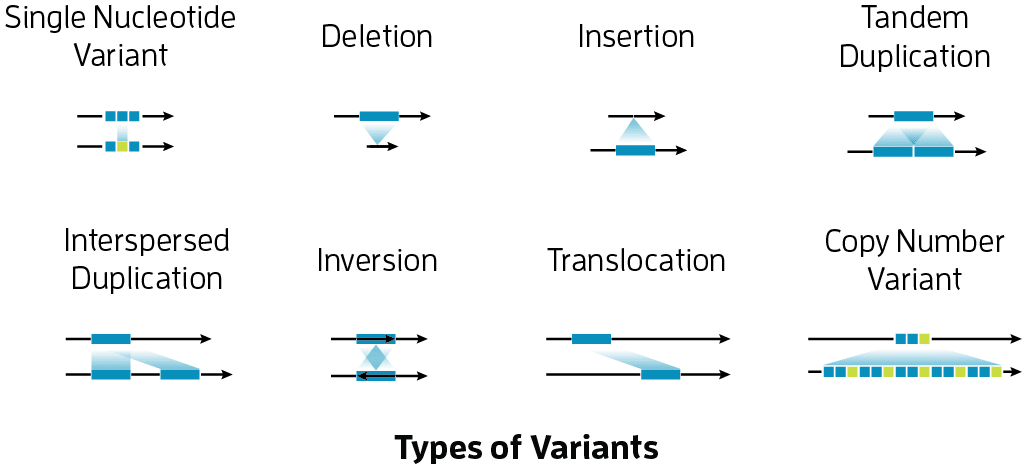
\includegraphics[width=0.7\textwidth]{img/splitthreader/variants}
	\caption{Example of structural variants. Source: \cite{sv_pacbio_2021}}
	\label{fig:variants}
\end{figure}

\subsubsection{Copy number variants}

.- According to the National Human Genome (NIH): ``A copy number variation (CNV) is when the number of copies of a particular gene varies from one individual to the next'' \cite{cnv_nih_2021}. For example in Figure \ref{fig:cnv}, we present some examples of CNV, we could see how the number of genes varies individual 2 to 6. Additionally, it is recognized that some cancer diseases are associated to CNV \cite{cnv_nih_2021, nattestad2016splitthreader, shlien2009copy, mitelman2007impact}.

\begin{figure}[H]
	\centering
	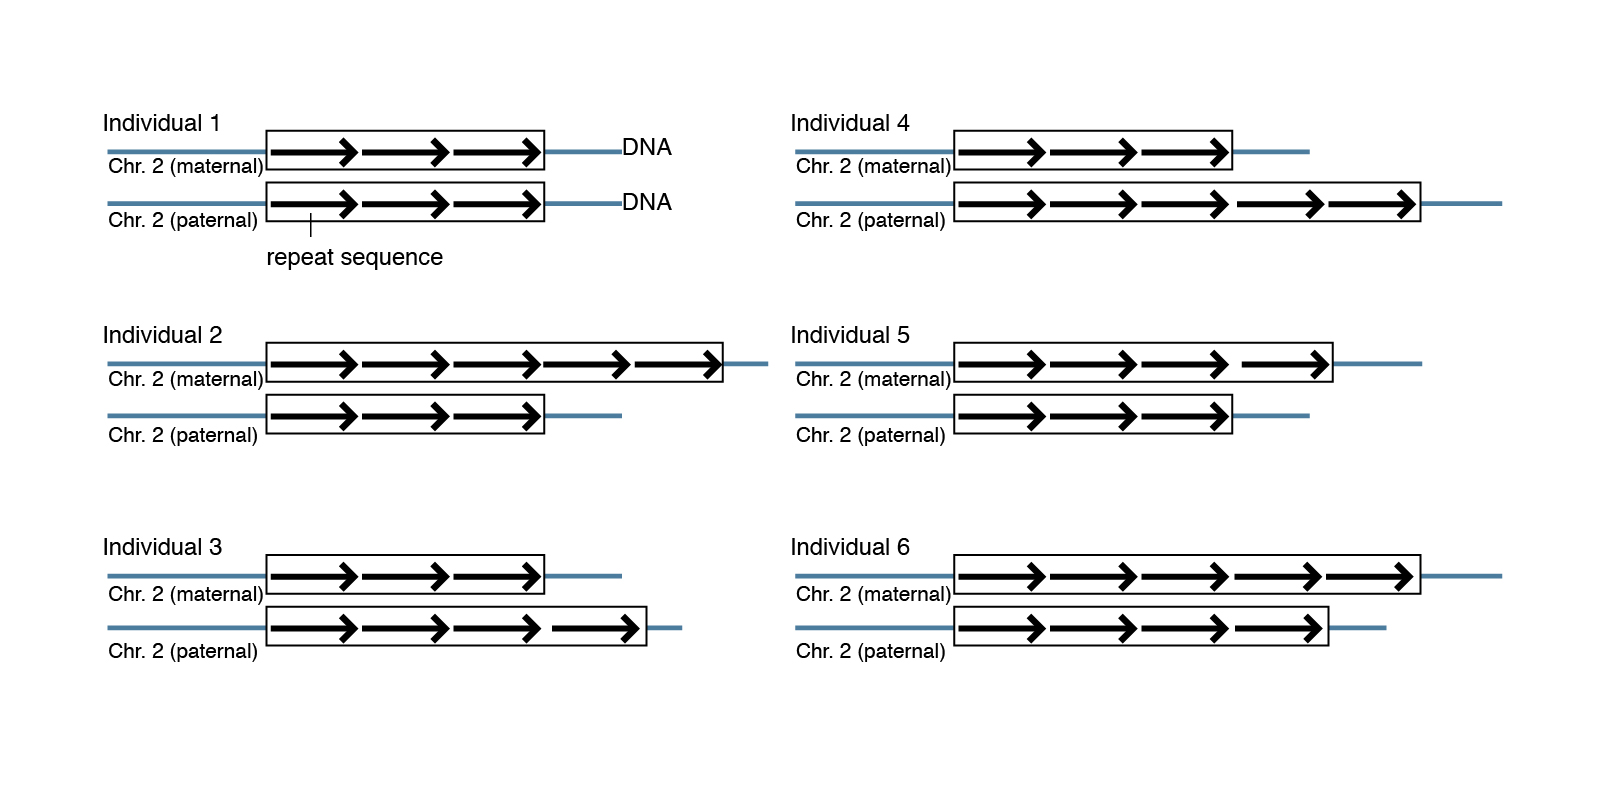
\includegraphics[width=0.8\textwidth]{img/splitthreader/copy_number_variation}
	\caption{Example of copy number variation. Source: \cite{cnv_nih_2021}}
	\label{fig:cnv}
\end{figure}



\subsubsection{Gene fusions}

.- Gene fusion is a gene made by two or more genes \cite{genefusion_nih_2021}. For example, the first gene
fusion discovered in cancer was BCR/ABL (related to leukemia), it is resulted from a fusion of chromosomes \cite{stam1985evidence}.

%%%%%%%%%%%%%%%%%%%%%%%%%%%%%%%%%%%%%%%%%%%%%%%%%%%%%%%%%%%%%%%%%%%%%%%%%%%%%%%%%%%%%
%%%%%%%%%%%%%%%%%%%%%%%%%%%%%%%%%%%%%%%%%%%%%%%%%%%%%%%%%%%%%%%%%%%%%%%%%%%%%%%%%%%%%
\section{Related work} 
%%%%%%%%%%%%%%%%%%%%%%%%%%%%%%%%%%%%%%%%%%%%%%%%%%%%%%%%%%%%%%%%%%%%%%%%%%%%%%%%%%%%%
%%%%%%%%%%%%%%%%%%%%%%%%%%%%%%%%%%%%%%%%%%%%%%%%%%%%%%%%%%%%%%%%%%%%%%%%%%%%%%%%%%%%%




%%%%%%%%%%%%%%%%%%%%%%%%%%%%%%%%%%%%%%%%%%%%%%%%%%%%%%%%%%%%%%%%%%%%%%%%%%%%%%%%%%%%%
%%%%%%%%%%%%%%%%%%%%%%%%%%%%%%%%%%%%%%%%%%%%%%%%%%%%%%%%%%%%%%%%%%%%%%%%%%%%%%%%%%%%%
\section{Proposal} 
%%%%%%%%%%%%%%%%%%%%%%%%%%%%%%%%%%%%%%%%%%%%%%%%%%%%%%%%%%%%%%%%%%%%%%%%%%%%%%%%%%%%%
%%%%%%%%%%%%%%%%%%%%%%%%%%%%%%%%%%%%%%%%%%%%%%%%%%%%%%%%%%%%%%%%%%%%%%%%%%%%%%%%%%%%%

In this work, we replicated the results of SplitThreader

%%%%%%%%%%%%%%%%%%%%%%%%%%%%%%%%%%%%%%%%%%%%%%%%%%%%%%%%%%%%%%%%%%%%%%%%%%%%%%%%%%%%%
%%%%%%%%%%%%%%%%%%%%%%%%%%%%%%%%%%%%%%%%%%%%%%%%%%%%%%%%%%%%%%%%%%%%%%%%%%%%%%%%%%%%%
\section{Results} 
%%%%%%%%%%%%%%%%%%%%%%%%%%%%%%%%%%%%%%%%%%%%%%%%%%%%%%%%%%%%%%%%%%%%%%%%%%%%%%%%%%%%%
%%%%%%%%%%%%%%%%%%%%%%%%%%%%%%%%%%%%%%%%%%%%%%%%%%%%%%%%%%%%%%%%%%%%%%%%%%%%%%%%%%%%%

%%%%%%%%%%%%%%%%%%%%%%%%%%%%%%%%%%%%%%%%%%%%%%%%%%%%%%%%%%%%%%%%%%%%%%%%%%%%%%%%%%%%%
%%%%%%%%%%%%%%%%%%%%%%%%%%%%%%%%%%%%%%%%%%%%%%%%%%%%%%%%%%%%%%%%%%%%%%%%%%%%%%%%%%%%%
\section{Conclusions} \label{section:conclusions}	
%%%%%%%%%%%%%%%%%%%%%%%%%%%%%%%%%%%%%%%%%%%%%%%%%%%%%%%%%%%%%%%%%%%%%%%%%%%%%%%%%%%%%
%%%%%%%%%%%%%%%%%%%%%%%%%%%%%%%%%%%%%%%%%%%%%%%%%%%%%%%%%%%%%%%%%%%%%%%%%%%%%%%%%%%%%



% ---- Bibliography ----
%\clearpage
\bibliographystyle{unsrt}
\bibliography{bibliography}

\end{document}
